\documentclass[12pt]{article}
\usepackage[margin=1in]{geometry} 
\usepackage{graphicx}
\usepackage{amsmath,amsthm,amssymb}
\usepackage{hyperref}

\title{
    \textbf{Programming Assignment 1} \\ 
    \textbf{CS5280} \\
}

\author{
    \textbf{Darpan Gaur} \\
    \textbf{CO21BTECH11004}
}


\date{}

\begin{document}
\maketitle

\hrulefill

\section*{Overview}
Implemented BOCC and FOCC-CTA using fine grained locking i.e., for operations read(), write() and tryCommmit() a lock on data-item and transaction is used, instead of a global lock.

\section*{Number of transactions}
Parameters used to generate the data:
$n=16$, $m=1000$, $numIters=20$, $constVal=1000$, $\lambda=20$, $numTrans = [1000, 2000, 3000, 4000, 5000]$
% plot two figure side by side
\begin{figure*}[h]
    \centering
    \begin{minipage}[b]{0.45\textwidth}
        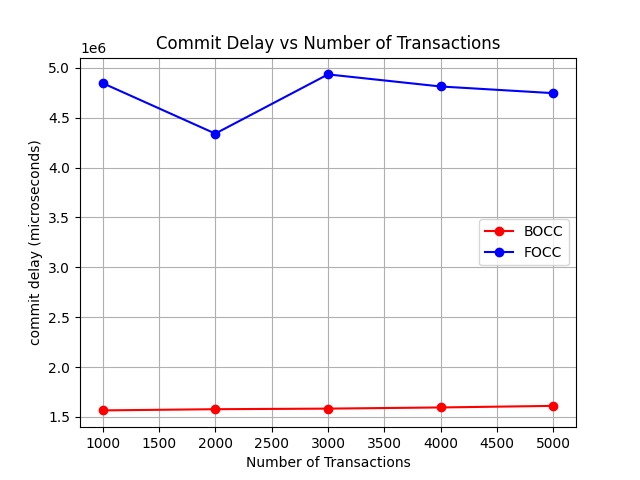
\includegraphics[width=\textwidth]{../code/commitDelayVsNumTrans.png}
        \caption{Commit delay vs Number of transactions}
    \end{minipage}
    \hfill
    \begin{minipage}[b]{0.45\textwidth}
        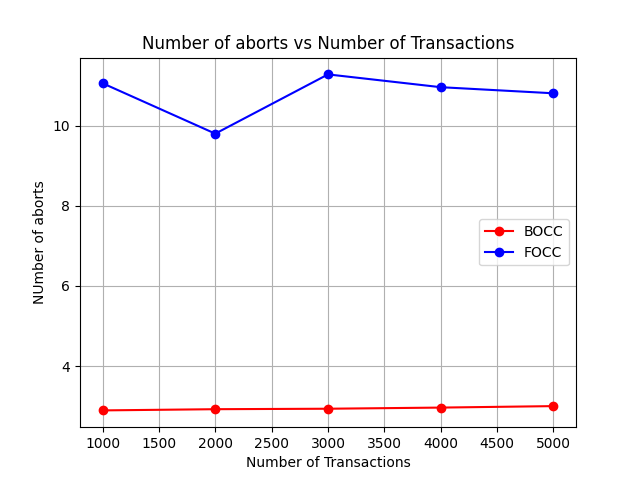
\includegraphics[width=\textwidth]{../code/numAbortsVsNumTrans.png}
        \caption{Number of aborts vs Number of transactions}
    \end{minipage}
\end{figure*}
\begin{itemize}
    \item FOCC-CTA has higher (approx three times) commit delay than BOCC for all number of transactions, as there are more number of aborts in FOCC-CTA.
    \item Commit delay is almost constant with increase in number of transactions for both BOCC and FOCC-CTA.
    \item FOCC-CTA has higher number of aborts than BOCC for all number of transactions.
    \item Number of aborts is also not varying much with increase in number of transactions for both BOCC and FOCC-CTA.
\end{itemize}

\section*{Number of variables}
Parameters used to generate the data:
$n=16$, $numTrans=1000$, $numIters=20$, $constVal=1000$, $\lambda=20$, $m = [1000, 2000, 3000, 4000, 5000]$

\begin{figure*}[h]
    \centering
    \begin{minipage}[b]{0.45\textwidth}
        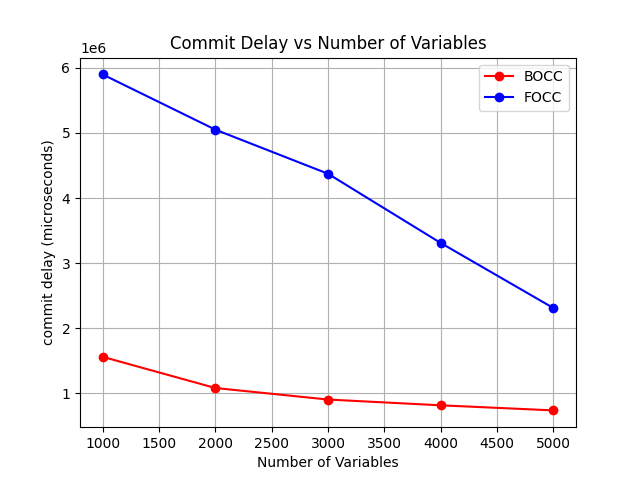
\includegraphics[width=\textwidth]{../code/commitDelayVsNumVars.png}
        \caption{Commit delay vs Number of variables}
    \end{minipage}
    \hfill
    \begin{minipage}[b]{0.45\textwidth}
        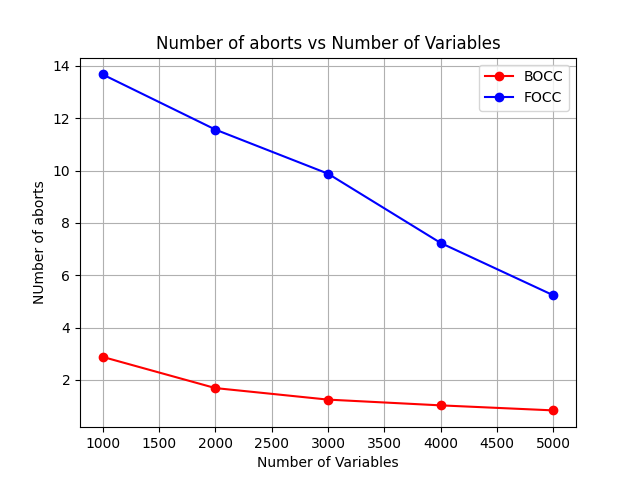
\includegraphics[width=\textwidth]{../code/numAbortsVsNumVars.png}
        \caption{Number of aborts vs Number of variables}
    \end{minipage}
\end{figure*}
\begin{itemize}
    \item FOCC-CTA has higher commit delay than BOCC for all number of variables, as there are more number of aborts in FOCC-CTA.
    \item Commit delay is decreasing with increase in number of variables for both BOCC and FOCC-CTA, as with more number of variables, conflicts are less, so less number of aborts.
    \item FOCC-CTA has higher number of aborts than BOCC for all number of variables.
    \item Number of aborts is decreasing with increase in number of variables for both BOCC and FOCC-CTA, as with more number of variables, conflicts are less, so less number of aborts.
\end{itemize}

\section*{Number of threads}
Parameters used to generate the data:
$n=16$, $m=1000$, $numTrans=1000$, $constVal=1000$, $\lambda=20$, $numIters = 20$, $numThreads = [2, 4, 8, 16, 32]$
\begin{figure*}[h]
    \centering
    \begin{minipage}[b]{0.45\textwidth}
        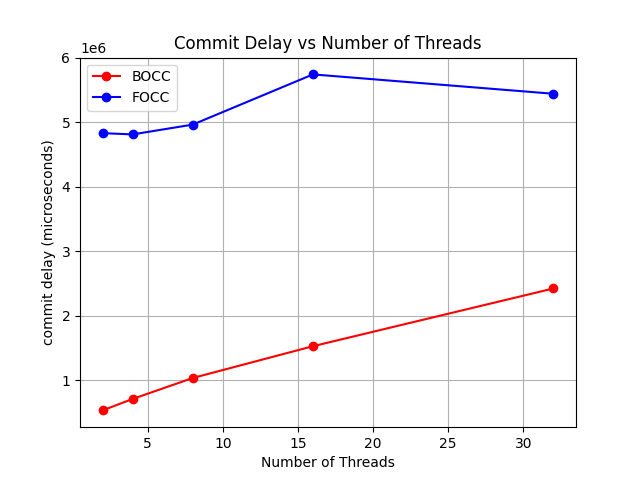
\includegraphics[width=\textwidth]{../code/commitDelayVsNumThreads.png}
        \caption{Commit delay vs Number of threads}
    \end{minipage}
    \hfill
    \begin{minipage}[b]{0.45\textwidth}
        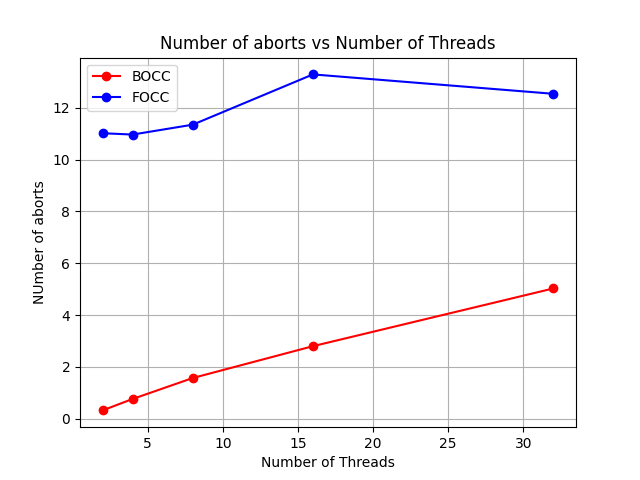
\includegraphics[width=\textwidth]{../code/numAbortsVsNumThreads.png}
        \caption{Number of aborts vs Number of threads}
    \end{minipage}
\end{figure*}
\begin{itemize}
    \item FOCC-CTA has higher commit delay than BOCC for all number of threads, as there are more number of aborts in FOCC-CTA.
    \item Commit delay increases with increase in number of threads for both BOCC and FOCC-CTA, as with more number of threads, more transactions are running concurrently, so more conflicts and more number of aborts.
    \item FOCC-CTA has higher number of aborts than BOCC for all number of threads.
    \item Number of aborts increases with increase in number of threads for both BOCC and FOCC-CTA, as with more number of threads, more transactions are running concurrently, so more conflicts and more number of aborts.
\end{itemize}

\end{document}